%%%%%%%%%%%%%%%%%%%%%%%%%%%%%%%%%%%%%%%%%%%%
\subsubsection{Measurement of Cobra Center Positions and Other Parameters [Daytime]}\label{secflow:CobraCal}

In this process, we measure the center position and other parameters of the fiber positioner ``Cobras".
In order for MPS to send commands for moving Cobras, MPS should should obtain firstly the following parameters (Figure \ref{fig:Cobraparams}):
\begin{itemize}
\item $\bm{X_{c,k}}=(x_{c,k}, y_{c,k})$ : center position of the positioner
\item $a_{1,k}$: arm lengths of $\theta$ stage
\item $a_{2,k}$: arm lengths of $\phi$ stage
\item $\bm{\theta _{\mathrm{CW},k}}$: CW limit of $\theta$ stage (angle or position)
\item $\bm{\phi _{\mathrm{CW},k}}$: CW limit of $\phi$ stage (angle or position)
\item $\bm{\theta _{\mathrm{CCW},k}}$: CCW limit of $\theta$ stage (angle or position), and
\item $\bm{\phi_{\mathrm{CCW},k}}$: CCW limit of $\phi$ stage (angle or position).
\end{itemize}
Note that these parameters are calculated in F3C.
We shall derive these parameters in this phase using back-illuminated fibers.

Prior to the measurement, we should confirm that the science fibers can be back-illuminated, that is, the Back Illumination Assembly in the SpS subsystem does work (see \ref{secflow:PFIon}, where we can do this step alternatively).
At this point, we regulate the brightness of back-illumination.
The brightness of back-illuminated fibers are set based on that of the science fibers illuminated in the strobe mode, whose brightness is fixed ($1 \; \mathrm{[W\;m^{-2} \; sr^{-1}]} \pm 20 \%$).
Firstly, we shall regulate the brightness the brightness of the fiducial fibers comparing with that of science fibers illuminated in the strobe mode.
Secondary, we shall adjust the brightness of science fibers back-lit in the normal mode to that of fiducial fibers. 

\smallskip

After tuning the brightness of the light sources, we shall back-illuminate the science fibers in the normal mode.
Firstly, we take fiber image without ``Cobra" moving for coordinate transformation.
We shall take fibers image using MCS in both short-exposure and long-exposure mode ($\sim 1$ second) with ``Cobra" rotating.
Because one MCS image has arcs of illuminated fibers, we combine the images, or use the spot positions which MCS measures.
We shall measure the centroid of the positioner, arm lengths, and minimum and maximum positions of each stage, by fitting the spots with a circle on F3C.
Here, we move $\theta$ and $\phi$ stage individually to determine these parameters.
The detailed procedure is presented in {\tt SSN-00021-001+-MPSconfiguration.pptx} (by Atsushi Shimono).

%We also check dependency of the offset of fiducial fiber positions at various RoA and El, although the offset is negligible given that PFI should be solid.
%If the displacement of the fiducial fibers is quite large and randomly, we should improve MCS--PFI relation, which is determined in the \ref{secflow:mcs2f3c} process.

Derived parameters are sent to MPS, which can move cobras everywhere at this point.
Then, we also validate the following items:
\begin{itemize}
\item If the SpS and Cable B are installed, the science fibers are moved to the home position several times to test good repeatability ($\sim$1um)
\item Dots can be obscure the Fibers.
We move the fibers to the dot positions and turn on the calibration lamp.
Take fibers image by MCS and compare with that of home position, where the fibers are not obscured.
If dots and "move-to-dot" command work, the spots in MCS is fainter than those with the fibers at home position.
\end{itemize}

Note that we should take care to avoid collisions in this process, although this depends on how much the cobra parameters will be updated by this calibration\footnote{We should take care about collision in the process \ref{secflow:FibID}, although the possibility is much less, because we will move a several fibers at a time.}.
According to the current schedule, Cobra parameters for SM1,2 will be calibrated at the run 2, while those for SM3,4 will be calibrated at the run 3.
Therefore, it is safe to set not-targeted Cobras around the home position, or inside enough before calibration.
Because three SMs expect for SM4 will be ready at the runs 2 and 3, we shall back-illuminate fibers of SM4 somehow (maybe illuminate from the Cable A).

To avoid contamination by neighboring Cobras, we separate 3 or 4 groups for calibration. 
We estimate 1-day for calibration of cobra parameters of SMs 1,2 and SMs 3,4 each.

%Cobras for SM1 and SM2 can be calibrated prior to those for SM3 and SM4.
%However, to avoid collisions between neighboring fiber positioners, ALL fibers are needed to back-illuminated.
%If the function of BIA for all SMs are confirmed, this sequence can be executed prior to \ref{secflow:P09}

\paragraph{Designated Took for This Process}
The tool is needed for measuring the centroid of the positioner, arm lengths, and minimum and maximum positions of each stage.
For coordinate transformation from MCS to F3C, we use the software module FPS (Fiber Positioning Sequencer).

%---------------------------------------
% Figure: Cobra parameters
%---------------------------------------
\begin{figure}[!ht]
\begin{center}
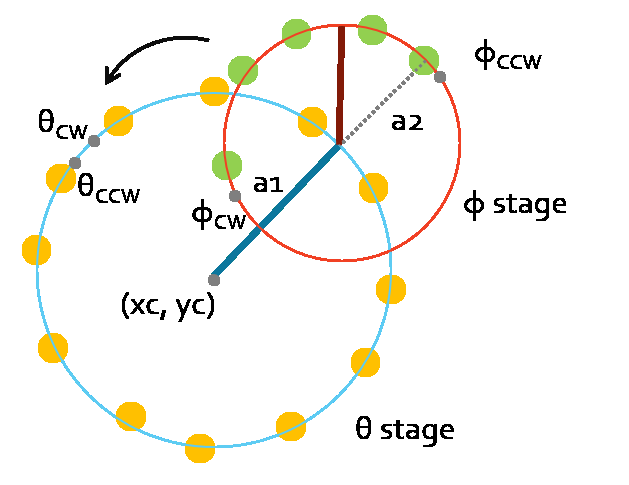
\includegraphics[width=75mm]{Calib_D3.eps}
\end{center}
\caption{Schematic picture of Cobra parameters.
Orange and green spots imply the positions of blinking fiber in F3C.
Light-blue and red circles indicate fitted circles for fiber spots.
}
\label{fig:Cobraparams}
\end{figure}


\begin{itembox}[l]{\suctitle{Success Criteria}}
The brightness of back-lit fibers are regulated. \\
Parameters of each Cobra $(x_{c,k}, y_{c,k}, a_{1,k}, a_{2,k}, \bm{\theta _{0,k}}, \bm{\theta _{m,k}}, \bm{\phi _{0,k}}, \bm{\phi _{m,k}})$ are measured and stored to MPS.

\bluetext{Required long time to analyze the data?: No. \\
--- We shall analyze the data in real-time.
In addition, cobra parameters will be stored in short time scale.
}
\end{itembox}